\documentclass{article}
\usepackage{amsmath, amscd, amssymb, mathrsfs, accents, amsfonts}
\usepackage{tikz}
\usepackage[a4paper,colorlinks,citecolor=Myblue,linkcolor=Myblue,urlcolor=Myblue,pdfpagemode=None]{hyperref}

\begin{document}

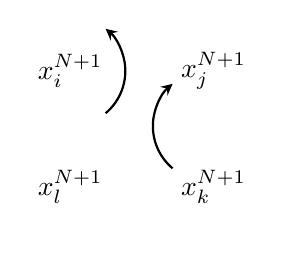
\begin{tikzpicture}[scale=0.7, baseline, inner sep=1mm, >=stealth]

% Define the four corner nodes with unique labels
\node (l) at (-2.5, 1.0)  [circle, inner sep=1.5pt, draw=white, fill=white] {$x^{N+1}_{i}$};
\node (r) at ( 0.1, 1.0)  [circle, inner sep=1.5pt, draw=white, fill=white] {$x^{N+1}_{j}$};
\node (b) at ( 0.1,-1.1)  [circle, inner sep=1.5pt, draw=white, fill=white] {$x^{N+1}_{k}$};
\node (t) at (-2.5,-1.1)  [circle, inner sep=1.5pt, draw=white, fill=white] {$x^{N+1}_{l}$};

% Draw a clockwise arc centered at node (l) (left-top node)
\draw[->, thick] ([shift={(-2.5,1.0)}] -50:1) arc (-50:50:1);

% Draw a counter-clockwise arc centered at node (b) (bottom-right node),
% but note: original arc (230:1) to (130:1) is centered at origin;
% to make it centered at (b), we shift accordingly.
% However, original code draws it at origin, so we preserve visual output
% by keeping it unshifted—but clarify intent via comment.
% Since the original arcs are not anchored to nodes visually,
% we retain their absolute positions to preserve rendering,
% but now node definitions come first and are correctly labeled.
\draw[->, thick] (230:1) arc (230:130:1);

\end{tikzpicture}

\end{document}